\chapter[ADNEX2: Updating the ADNEX model]{ADNEX2: Updating the ADNEX model to predict ovarian cancer for
surgically and conservatively managed patients with an adnexal mass}
\label{sec:chp_ADNEX2}


\begin{flushleft}
{\huge\sffamily \textbf{IN PREPARATION}}
\end{flushleft}
as:
\begin{quote}
\textbf{Barreñada L}, Froyman W, Ceusters J, Landolfo C, Wynants L, Ledger A, Sladkevicius P, Testa AC, Van Holsbeke C, Buonomo F, Kudla MJ, Fruscio R, Fischerova D, Franchi D, Epstein E, Chiappa V, Leone FPG, Ensor J, Coccia ME, Guerriero S, Alcazar JL, Alves F, Jokubkiene L, Pozzati F, Moro F, Mascilini F, Taliento C, Bourne T, Valentin L, Timmerman D, Van Calster B. ADNEX2: Updating the ADNEX model to predict ovarian cancer for surgically and conservatively managed patients with an adnexal mass. \textit{In preparation}. \textbf{The content of this chapter is therefore not final and may change in the future}.
\end{quote}

\begin{quote}
\textbf{Preliminary supplementary material and code} available at \url{https://osf.io/36n8m/overview?view_only=0f1fa6d9a5e34e4d901c05922d0d0307}.
\end{quote}
\vspace{0.2em}
\noindent\scriptsize\textit{Presented at ISUOG 2025 in Cancun, Mexico}
\vspace{-0.5em}
\normalsize\vspace{-0.5em}

\section*{Summary}\label{abstract}

We updated the \gls{ADNEX} risk prediction model to ADNEX2 using data from 6,847 patients in the IOTA5 multicentre prospective cohort (17 centres, recruited 2012–2016), including both surgically managed and conservatively followed cases and excluding masses classifiable with the benign descriptors (BDs). Updating combined multinomial logistic recalibration with Bayesian refitting using random centre intercepts, and missing data were handled with multiple imputation; validation used leave-centre-out internal-external cross-validation. ADNEX2 was developed on 4,657 patients for whom the BDs did not apply; in the full sample the two-step strategy (BDs followed by ADNEX2, using CA125 when available) yielded an AUC of 0.95 (95\% CI 0.93–0.96), and in the development subset ADNEX2 achieved an AUC of 0.93 (0.91–0.94). ADNEX2 improves calibration over the original model and is intended for use after applying the BDs; CA125 is not essential for the referral decision but is recommended when assessing likely malignant subtype.

\vspace{0.5cm}

\newpage

\section{Introduction}

When confronted with an ovarian tumour, clinical staff has to decide on the appropriate management. The optimal management depends on the type of tumour. Most benign tumours can be followed up conservatively, whereas different types of malignant tumours require different treatment. The \gls{ADNEX} model is a mathematical model to estimate the likelihood of different tumour types: benign, borderline malignant, stage I primary invasive, stage II-IV primary invasive, and secondary metastasis \cite{vancalsterEvaluatingRiskOvarian2014}. \gls{ADNEX} includes three clinical and six ultrasound variables. It has one version with serum \gls{CA125} as a predictor and another one without. The other predictors are age, type of centre at which the ultrasound examination was performed (oncology centre vs other) and the following ultrasound variables: maximum diameter of the lesion, proportion of solid tissue, number of papillations, more than 10 cyst locules, ascites, and acoustic shadows. Type of centre is included to acknowledge differences in prevalence of malignant tumours between centres. \gls{ADNEX} is intended to be used by clinicians after ultrasound examination of a patient with an adnexal mass to assess the risk of the mass being malignant. According to an international consensus document, masses judged to be almost certainly benign (\gls{ADNEX} risk lower than 1\%) can be managed with clinical and ultrasound follow up. If malignancy risk is between 1 and 10\%, the tumour can be surgically managed in a general gynaecology unit. If risk of malignancy is 10\% or higher, the patient should be referred to a gynaecologic oncology specialist, and the risk of each malignant tumour subtype can then be used to help decide the type of surgical treatment \cite{timmermanESGOISUOGIOTA2021}.

Nevertheless, \gls{ADNEX} can be improved for three reasons. First, the model was based on patients recruited between 1999 and 2012 (\gls{IOTA} phases 1--3), i.e., 14 to 27 years ago. Populations are bound to change over time, which may negatively affect model performance \cite{vancalsterThereNoSuch2023}. Retraining models on more recent data, if possible, is therefore of interest. Second, like nearly all studies in the field, the \gls{ADNEX} development study included only patients that underwent surgery. While this approach allows the tumour outcome to be based on a reliable reference standard (histopathology), it suffers from selection bias by not including ovarian masses that are not operated on. This is problematic for all available models: while these model are developed to support the decision to operate or not, model development samples excluded patients where the eventual decision was to not operate. Third, there is strong evidence that a large proportion of tumours can be classified as benign without a mathematical model by using the \glspl{BD}. A two-step strategy has been proposed, where first the \glspl{BD} are used and then \gls{ADNEX} is applied to the tumours where no \gls{BD} applies \cite{landolfoBenignDescriptorsADNEX2023}. A prospective multicenter validation indicated that the \glspl{BD} can be used in 37\% of patients, of which 99.3\% had a benign tumour. This approach has been validated seven times, showing similar performance  \cite{barcroftEvaluatingUseTwostep2024,borgesProspectiveExternalValidation2024, devitisDiagnosticAlgorithmsAdnexal2025, einigExternalValidationIOTA2025, pascualValidationADNEXIOTA2024,perryCostConsequenceAnalysis2026, timmermanExternalValidationOvarianAdnexal2023}. Hence, it makes sense to update \gls{ADNEX} only on data from patients for whom the \gls{BD} does not apply.

The objective of this study is to update the \gls{ADNEX} model on recent data from patients that underwent surgery or were followed conservatively and with tumours to which the \glspl{BD} did not apply, and to validate the model. Such an updated model should be better suited for use in a two-step strategy, where application of the \glspl{BD} is the first step.

\section{Methods}

\subsection{Design and participants}

We use data from the \gls{IOTA} 5 study, an ongoing multicentre prospective cohort study including patients with an adnexal mass managed with surgery or with clinical and ultrasound follow-up. Patients were recruited between 1st January 2012 and 31st December 2016 \cite{timmermanIOTAPhase52025}. Conservatively managed patients included here were followed up until 31st December 2022. Inclusion criteria were being at least 18 years old and presenting with at least one adnexal mass (ovarian, para-ovarian, or tubal) at recruitment. Exclusion criteria were having a lesion presumed to be physiological with a largest diameter less than 3~cm or refusing or withdrawing informed consent. Pregnancy was not an exclusion criterion. We also excluded patients with a mass that was already in follow-up at the recruitment centre before recruitment into the study.

Patients were recruited at 39 oncology and non-oncology centres across 15 countries, with oncology centres defined as centres with a dedicated gynaecologic oncology unit. For this study, we use data on 6847 patients recruited at 17 centres. These 17 centres satisfied predefined quality criteria and aimed to consecutively recruit patients selected for surgery or for management with clinical and ultrasound follow-up (Figure~\ref{fig:ADNEX2:1}; criteria for excluding centres are described in Supplementary material S1). The IOTA5 study was approved by the Research Ethics Committee from the University Hospitals KU Leuven as the coordinating centre (B32220095331/S51375), and by local ethics committees of all participating centres. We reported the study according to the \gls{TRIPOD}+\gls{AI} guideline \cite{collinsTRIPODAIStatementUpdated2024}.

\subsection{Procedures and variable measurements}

Patients were recruited by ultrasound examiners. The ultrasound examiners were gynaecologists with expertise in gynaecological ultrasound. They were either \gls{IOTA} trainers or had passed the \gls{IOTA} certification test. When recruiting, the ultrasound examiners followed a standardised research protocol (\url{https://clinicaltrials.gov/study/NCT01698632}). Standardized clinical information was collected and a standardised transvaginal ultrasound examination was performed supplemented with abdominal ultrasound if necessary. The recruitment examination included scanning the uterus, both adnexa, and the whole pelvis outside these organs. Grey scale and colour or power Doppler ultrasound was used to characterise the morphology and vascularisation of each adnexal mass. Information on a set of predefined ultrasound variables, including those used in the \gls{ADNEX} model, was collected, and the \gls{IOTA} terminology was used to describe the ultrasound findings \cite{timmermanTermsDefinitionsMeasurements2000}. In addition, the ultrasound examiners provided a diagnosis based on their subjective assessment by classifying each lesion as benign, borderline, or malignant, and by specifying the degree of certainty of their classification (certain, probable, or uncertain). Based on pattern recognition they also suggested a specific histology for each mass choosing from a list of 18 predefined diagnoses \cite{valentinUseMorphologyCharacterize2004}.

When multiple adnexal masses were found on ultrasound, the dominant mass was included in the statistical analysis. The dominant mass was the mass with the most complex ultrasound morphology. If multiple masses had similar morphology, the largest mass or the mass that was most easily accessible with ultrasound was denoted dominant. We encouraged centres to measure the patients' serum \gls{CA125} level, but this was not a requirement for inclusion in the study. Measurement of \gls{CA125} was left to clinical judgement and local protocols. Due to the prospective study design, predictor measurements were blinded to tumour outcome.

Based on patient history, clinical and ultrasound findings, the ultrasound examiner suggested surgery or conservative management with follow-up. The final decision on management was made by the treating physician in dialogue with the patient. Conservative management included ultrasound and clinical follow-up at intervals of three months, six months, and then every 12~months thereafter. At follow-up visits clinical information, including symptoms, was collected, an ultrasound examination was performed and the same standardized ultrasound information as at the inclusion scan was collected. After one or more follow-up visits, some patients underwent surgery for a variety of reasons (e.g., suspicion of malignancy or patient anxiety) \cite{froymanRiskComplicationsPatients2019}. For some patients, the mass resolved spontaneously during follow-up. Each centre performed surgery by following local protocols and histological examination of surgically removed masses.

\subsection{Outcome}

Patients who were managed conservatively were followed up until the first occurrence of one of the following events: the mass resolved spontaneously, the mass was surgically removed, the patient died, or the date was 31 December 2022. The outcome describes the nature of the adnexal mass at inclusion (benign, borderline, stage I primary invasive, Stage II-IV primary invasive, or secondary metastasis). The primary outcome is classification of tumours as benign or malignant at inclusion. This classification is based on histology when patients underwent surgery, or on subjective assessment of ultrasound images at inclusion and during follow-up until 12~($\pm 2$)~months if surgery was not performed \cite{vancalsterValidationModelsDiagnose2020}. If there was insufficient information to make a reasonable classification of the nature of the mass at inclusion the outcome was classified as uncertain.

Pathologists were blinded to ultrasound predictor variables and model predictions but might have received information on subjective assessment by the ultrasound examiner when clinically relevant. Borderline tumours were classified as malignant. Central pathology review was not done because in a previous study we did not observe important differences in reported outcomes between local and central pathology reports \cite{timmermanLogisticRegressionModel2005}. The stage of the malignant tumours was determined using the criteria by the International Federation of Gynaecology and Obstetrics (FIGO) \cite{heintzCarcinomaOvary2003}.

\subsection{Data cleaning and preparation}

Patient data was collected using a study-specific secure electronic platform (Astraia software, Munich, Germany), and encrypted data communication to ensure data security. As of 01/01/2022, data were collected through a different but similar platform, Clinical Data Miner (CDM) \cite{installeClinicalDataMiner2014}. A team of biostatisticians and ultrasound examiners performed data cleaning through regular meetings and by sending queries to participating centres to retrieve missing information or to correct inconsistencies.

\subsection{Statistical analysis}

We compared the available sample size with Pate et al.'s sample size criteria for multinomial logistic regression prediction models \cite{pateMinimumSampleSize2023} (details in Supplementary material S2.1). We followed a prespecified statistical analysis plan for this study preregistered in \gls{OSF} (\url{https://osf.io/36n8m/overview?view_only=0f1fa6d9a5e34e4d901c05922d0d0307}).

Missing values occurred for \gls{CA125} and the outcome (when labelled as uncertain), and were handled with multiple imputation (Table S4; details in Supplementary material S2.2). 

ADNEX without \gls{CA125} and ADNEX with \gls{CA125} were updated on the dataset of patients with tumours to which the \glspl{BD} did not apply. We used the following procedure to obtain ADNEX2. We used the same predictors and transformations (for continuous predictors) as in \gls{ADNEX}. First, we fitted a multinomial logistic recalibration model to update intercepts and coefficients using slopes \cite{vancalsterValidationUpdatingRisk2017}. In the second step, we used Bayesian refitting using information from the original \gls{ADNEX} model and the logistic recalibration \cite{suReviewStatisticalUpdating2018,vandeschootBayesianStatisticsModelling2021}. In both steps, we used models with random intercepts per centre \cite{wynantsDoesIgnoringClustering2018}. Details on the model updating procedure are found in supplementary material S2.3.1.

To validate the two-step strategy, patients with tumours to which the \glspl{BD} applied were assigned risk estimates for the five outcome categories. These estimates were obtained as the prevalence of each outcome category in the subgroup of patients with tumours to which the BDs applied, averaged over the 100 imputed datasets

We validated the two-step strategy and ADNEX2 (with and without \gls{CA125}) using internal-external cross-validation (IECV) to estimate how the model would perform in new centres \cite{collinsEvaluationClinicalPrediction2024, roystonConstructionValidationPrognostic2004}. Internal-external cross-validation mimics geographical external validation by treating every centre once as a test set for models developed on the remaining 16~centres. The approaches to update ADNEX2 and to generate risk estimates when the \glspl{BD} apply were implemented on data from 16~centres and tested on data from the remaining centres. To validate ADNEX2 with \gls{CA125}, in isolation or as part of the two-step strategy, we used a realistic approach by using ADNEX2 with \gls{CA125} when \gls{CA125} was available and ADNEX without \gls{CA125} when \gls{CA125} was not available.

We present centre-specific results of the IECV procedure, as well as overall results using meta-analysis of centre-specific results, similar to previous work \cite{erikssonUltrasoundbasedRiskModel2020,vancalsterEvaluatingRiskOvarian2014}. 95\% \glsentryshort{CI}s are reported. Heterogeneity in performance between centres is quantified with \glsentryshort{PI}s \cite{partlettRandomEffectsMetaanalysis2017}. We report diagnostic performance for distinguishing benign from malignant tumours as follows: distribution of estimated risk per outcome category, area under the \glsentryshort{ROC} curve (\glsentryshort{AUC}), flexible centre-specific and overall calibration plots for the overall estimated risk of malignancy, and net benefit with decision curves for a decision threshold of 1\% (to decide whether conservative management should be considered) and for decision thresholds between 5 and 40\% (to decide whether the patient requires specialised care) on the estimated risk of malignancy \cite{barrenadaClusteredFlexibleCalibration2026,debrayFrameworkMetaanalysisPrediction2019,vancalsterPerformanceEvaluationPredictive2024,wynantsRandomeffectsMetaanalysisClinical2018}. Sensitivity, specificity, positive predictive value and negative predictive value for the same decision thresholds were also calculated. We report diagnostic performance for discriminating between the five subtypes of adnexal masses as \gls{PDI}, pairwise \glsentryshort{AUC}s and flexible calibration plots. Methodological details about the performance measures are available in Supplementary material S2.3.

We analysed performance for pre-specified subgroups: (1) postmenopausal versus premenopausal patients, (2) oncology centres versus other centres, and (3) patients that were operated within 120~days after inclusion scan. In the subgroups, only results for the two-step strategy are shown.

\subsection{Independent external validation}

The recalibrated and refitted coefficients of ADNEX2 are not shown because they will be included in a CE-labelled app offered by Gynaia Inc. (\url{https://www.gynaia.com/}). Members of the ovarian programme of Gynaia will have access to the app to use it as a decision support tool.

Researchers that aim to externally validate the model can do it by using \texttt{evaluatr} R package (in development). This package provides a safe environment for model developers and model evaluators where the developer does not have access to the patient data, and the evaluator does not have access to the model coefficients but can obtain a vector of predicted risks to evaluate the model's aggregate performance. Access to the model is given case by case, upon reasonable request to the model developers.

\begin{figure}
\centering
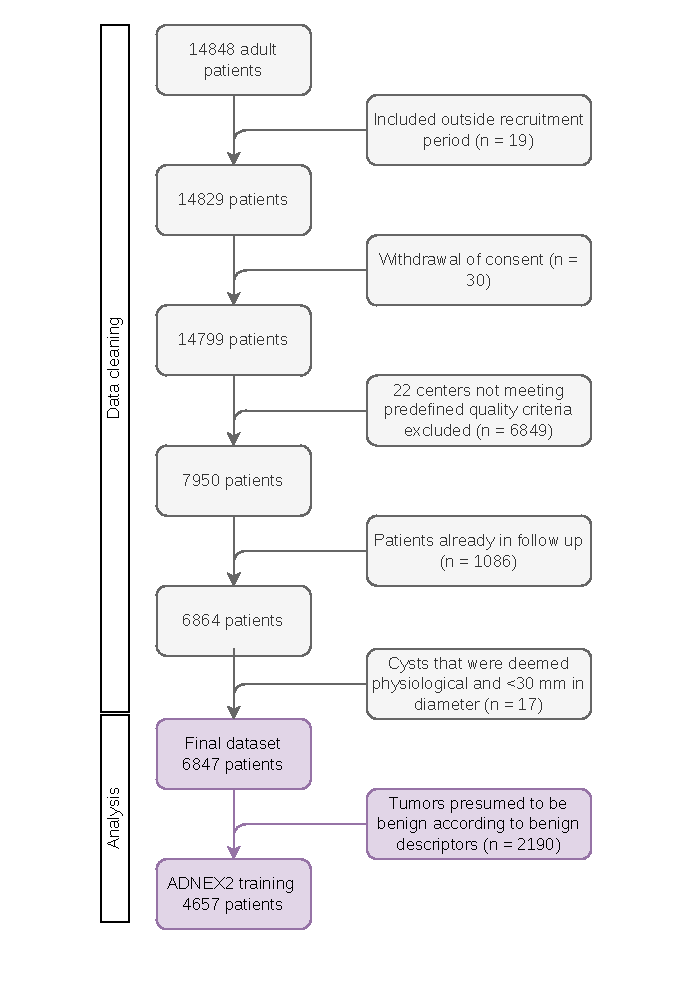
\includegraphics[width=0.8\textwidth]{figures/ADNEX2/PatientFlowDiagram_cropped.pdf}
\caption{Patient flow diagram of IOTA5 second interim analysis.}
\label{fig:ADNEX2:1}
\end{figure}

\begin{table}
\scriptsize
\centering
\caption{Descriptive statistics of the IOTA5 study cohorts.}
\label{tab:ADNEX2:1}
   \begin{tabularx}{\textwidth}{XXXX}
    \toprule
       \textbf{Variable} & \textbf{BD apply}  & \textbf{BD do not apply} & \textbf{All patients} \\ 
        \midrule
        \textbf{Number of cases} & 2190 & 4657 & 6847 \\ 
        \quad Benign & 1987 (91\%) & 2638 (57\%) & 4625 (68\%) \\ 
        \quad Borderline & 4 (0.2\%) & 387 (8\%) & 391 (6\%) \\ 
        \quad Stage I invasive cancer & 2 (0.1\%) & 301 (6\%) & 303 (4\%) \\ 
        \quad Stage II-IV invasive cancer & 2 (0.1\%) & 785 (17\%) & 787 (11\%) \\ 
        \quad Secondary Metastasis & 2 (0.1\%) & 227 (5\%) & 229 (3\%) \\ 
        \quad Uncertain\textsuperscript{a} & 193 (9\%) & 319 (7\%) & 512 (7\%) \\ 
        Surgery without follow up scan within 120 days after first scan & 726 (33\%) & 3174 (68\%) & 3900 (57\%) \\ 
        Patient age at recruitment (years)\textsuperscript{b} & 42 (32–54) [18–98] & 54 (41–66) [18–99] & 50 (37–63) [18–99] \\ 
        Postmenopausal & 656 (30\%) & 2646 (57\%) & 3302 (48\%) \\ 
        Pelvic pain & 394 (18\%) & 594 (13\%) & 988 (14\%) \\ 
        Presence of solid components & 0 (0\%) & 2801 (60\%) & 2801 (41\%) \\ 
        Proportion of solid components\textsuperscript{b} & 0 (0–0) [0–0] & 0.25 (0–0.81) [0–1] & 0 (0–0.49) [0–1] \\ 
        Maximum diameter of the lesion (mm)\textsuperscript{b} & 45 (32–61) [7–99] & 65 (43–105) [7–751] & 56 (39–87) [7–751] \\ 
        CA125 (U/ml) \textsuperscript{b} & 15 (9–30) [1–7745] & 35 (14–184) [1–78200] & 27 (12–127) [1–78200] \\ 
        CA125 missing  & 1498 (68\%) & 1728 (37\%) & 3226 (47\%) \\ 
        Shadows\textsuperscript{b} & 378 (17\%) & 926 (20\%) & 1304 (19\%) \\ 
        Ascites\textsuperscript{b} & 8 (0.4\%) & 482 (10\%) & 490 (7\%) \\
        \multicolumn{4}{l}{\textbf{Number of papillations\textsuperscript{b}}} \\ 
        \quad None & 2190 (100\%) & 3677 (79\%) & 5867 (85\%) \\ 
        \quad 1 & 0 (0\%) & 464 (10\%) & 464 (6\%) \\ 
        \quad 2 & 0 (0\%) & 143 (3\%) & 143 (2\%) \\ 
        \quad 3 & 0 (0\%) & 95 (2\%) & 95 (1\%) \\ 
        \quad 4 or more & 0 (0\%) & 278 (6\%) & 278 (4\%) \\ 
        More than 10 cyst locules\textsuperscript{b} & 0 (0\%) & 634 (14\%) & 634 (9\%) \\ 
        \multicolumn{4}{l}{\textbf{Colour score of intratumoral flow}} \\ 
        \quad 1: No blood flow & 1574 (72\%) & 1263 (27\%) & 2837 (41\%) \\ 
        \quad 2: minimal blood flow & 449 (21\%) & 1314 (28\%) & 1763 (26\%) \\ 
        \quad 3: moderate blood flow & 161 (7\%) & 1376 (30\%) & 1537 (22\%) \\ 
        \quad 4: very strong flow & 6 (0.3\%) & 704 (15\%) & 710 (10\%) \\ 
        \multicolumn{4}{l}{\textbf{Tumour type using IOTA terminology}} \\ 
        \quad Unilocular & 2190 (100\%) & 388 (8\%) & 2578 (38\%) \\ 
        \quad Unilocular solid & 0 (0\%) & 630 (13\%) & 630 (9\%) \\ 
        \quad Multilocular & 0 (0\%) & 1438 (31\%)               & 1438 (21\%)               \\ 
        \quad Multilocular solid & 0 (0\%) & 1111 (24\%)                & 1111 (16\%)                \\ 
        \quad Solid & 0 (0\%) & 1060 (23\%)                  & 1060 (15\%)                  \\ 
        \quad Not possible to classify & 0 (0\%) & 30 (1\%) & 30 (<1\%) \\ \bottomrule
    \end{tabularx}
\par\noindent\makebox[\textwidth][l]{%
\begin{minipage}[t]{\textwidth}
\addlinespace[0.5em]
\raggedright\footnotesize
Results are presented as median (IQR) [range] for continuous variables, or N (\%) for categorical variables. 

\textsuperscript{a}The outcome for uncertain tumours was imputed with multiple imputation. Tumours are uncertain if there was insufficient information to make a reasonable classification of the nature of the mass at inclusion.

\textsuperscript{b}ADNEX and ADNEX2 predictors.
\end{minipage}%
}
\end{table}

\section{Results}

After exclusions and data cleaning, 6847 patients recruited at 17~centres were included in the analysis (Figure~\ref{fig:ADNEX2:1}, Table S1, Supplementary material S1). The median age was 50~years (interquartile range 37--63) and 3302~patients (48\%) were postmenopausal (Table~\ref{tab:ADNEX2:1}). The tumour was benign in 4625 (68\%) patients, malignant in 1710~patients (25\%), and uncertain in 512 (7\%) patients. Of the malignant tumours, 391 (6\%) were borderline, 303 (4\%) stage I primary invasive, 787 (12\%) stage II--IV primary invasive, and 229 (3\%) secondary metastatic. The \glspl{BD} applied to 2190/6847 (32\%) tumours. The sample of 4657~patients with tumours to which a \gls{BD} did not apply was the development cohort for ADNEX2. Here, median age was 54~years (interquartile range 41--66), and 2646~patients (57\%) were postmenopausal (Table~\ref{tab:ADNEX2:1}). 2638~patients (57\%) had a benign tumour, 1700 (37\%) a malignant tumour, and 319 (7\%) a tumour of uncertain outcome. The serum \gls{CA125} levels was missing in 1728~patients (37\%). 3174~patients (68\%) underwent surgery without a follow-up scan. Further information on tumour outcome, missing CA125 values, and management decisions is provided in Tables S5-S10. 

Table S11 provides descriptive statistics of the 4657 patients on which ADNEX2 was developed and the 5909 patients on which ADNEX was developed.[LV48.1] The main difference between both cohorts was the higher proportion of unilocular tumours in ADNEX (30\%) with respect to ADNEX2 (8\%) and the higher presence of shadows with 13\% in ADNEX and 20\% in ADNEX2 (Table S11). 

\subsection{Benign descriptors}

2180 of the 2190 tumors for which a BD applied (99.5\%) were benign or had an uncertain outcome, 10 (0.5\%) were malignant (4 borderline, 2 stage I invasive, 2 stage II-IV invasive, 2 secondary metastatic) (Table S5). After multiple imputation of uncertain outcomes, 99.45\% tumours (99.1\% - 99.8\%[BV50.1][LB50.2]) were benign, 0.21\% (0.01\% - 0.42\%) borderline, 0.10\% (<0.01\% - 0.25\%) stage I primary invasive, 0.12\% (<0.01\% - 0.28\%) stage II-IV primary invasive, and 0.11\% (<0.01\% - 0.26\%) secondary metastatic (Table S6). 

\subsection{ADNEX2}

Figures S4-S6 present histograms of the predictions of the 6 validations per binary outcome and Figures S7-S9 the risk distribution per tumour subtype. The median highest estimated risk was always the true outcome, except for metastatic cancers in the model without CA125 where Stage II-IV and metastatic had similar estimated risks. The relation between predicted risks and variables was very similar for ADNEX and ADNEX2 (Figures S10-S11) but ADNEX2 tended to predict higher risks of malignant subtypes, especially borderline and metastatic cases (Figures S12-S13).  

\subsection{Discrimination}

The \gls{AUC} to discriminate between benign and malignant tumours in all patients was 0.94 (95\% \gls{CI} 0.93--0.95, 95\% \gls{PI} 0.89--0.98) for the two-step strategy using ADNEX2 without \gls{CA125} and 0.95 (95\% \gls{CI} 0.93--0.96, 95\% \gls{PI} 0.90--0.98) for the two-step strategy using ADNEX2 with \gls{CA125} if available (Table~\ref{tab:ADNEX2:2}, Table S12, Figure S14). On the patients for which the \glspl{BD} did not apply, the \gls{AUC} was 0.92 (0.90--0.93) for ADNEX2 without \gls{CA125} and 0.93 (0.91--0.94) for ADNEX2 with \gls{CA125} if available. The \glsentryshort{AUC}s for \gls{ADNEX} and ADNEX2 whether used alone or in a two-step strategy were similar. Using ADNEX2 with \gls{CA125} if available slightly improved \gls{AUC} over the version without \gls{CA125}. Forest plots with centre-specific performance are shown in Figures S15-S26. 

ADNEX2 with \gls{CA125} if available performed better than ADNEX2 without \gls{CA125} to discriminate stage II-IV primary invasive from other malignant subtypes (Table~\ref{tab:ADNEX2:3}). Importantly, ADNEX2 discriminated better than \gls{ADNEX} between borderline and stage I tumours.

\begin{figure}
\centering
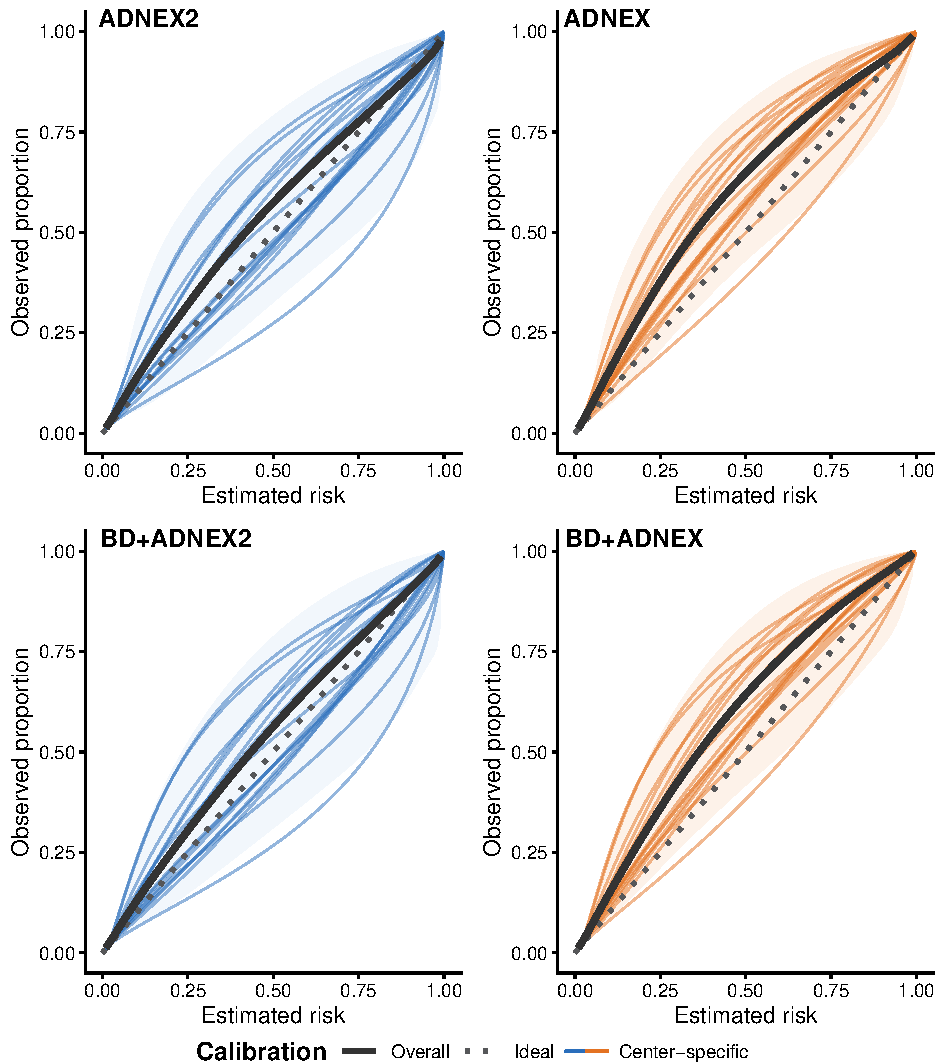
\includegraphics[width=0.8\textwidth]{figures/ADNEX2/Figure2clusteredcal.pdf}
\caption[Clustered calibration curves for ADNEX2 and ADNEX without CA125]{Clustered calibration curves for ADNEX2 without CA125 and ADNEX without CA125 if benign descriptors do not apply (n = 4657), and the two-step strategy with ADNEX2 without CA125 and the two-step strategy with ADNEX without CA125 in all patients (n = 6847). The shaded blue and orange area indicate the 95\% prediction interval for the calibration.}
\label{fig:ADNEX2:2}
\end{figure}

\subsection{Calibration}

ADNEX2 was well calibrated and showed better calibration than \gls{ADNEX} for predicting risk of malignancy whether used alone or in a two-step strategy. However with slightly wider prediction intervals (Figure~\ref{fig:ADNEX2:2}, Figures S27-S38). \gls{OE} ratios were between 1.03 and 1.05 for ADNEX2 and between 1.11 and 1.16 for \gls{ADNEX} (Table~\ref{tab:ADNEX2:2}, Table S13). This reflects the better calibration for ADNEX2: ADNEX2 underestimated risks less than \gls{ADNEX} (3 to 5\% versus 11 to 16\%). Calibration plots for each of the tumor subtypes confirmed that ADNEX2 was better calibrated than \gls{ADNEX} (Figures S39-S42). . 

\subsection{Classification and clinical utility}

When using the two-step strategy with ADNEX2, the 10\% risk of malignancy threshold yielded sensitivity 93\% and specificity 83--84\%, irrespective of whether ADNEX2 without \gls{CA125} or ADNEX2 with \gls{CA125} if available was used (Table~\ref{tab:ADNEX2:2}). Using the 1\% threshold, sensitivity was 97\% and specificity 52\% irrespective of whether ADNEX2 was used with or without \gls{CA125} (Table S14). The classification performance when using \gls{ADNEX} was similar with sometimes slightly lower sensitivity and slightly higher specificity.

The two-step strategy with ADNEX2 and that with \gls{ADNEX} had similar net benefit for decision thresholds up to around 10\% (Figure~\ref{fig:ADNEX2:3}, Figures S43 and S44). At 1\% decision threshold the models showed benefit but no or minimal utility with respect to the decision of treat all patients. The models were clinically useful for the rest of decision thresholds. At decision thresholds from 15\% to 35\%, using ADNEX2 instead of \gls{ADNEX} in the two-step strategy had higher net benefit. At higher thresholds ADNEX2 had higher net benefit only when \gls{CA125} was not used (Table~\ref{tab:ADNEX2:2}, Table S15, Figures S43 and S44). The meta-analysis estimated that, at the 10\% threshold, the two-step strategy with ADNEX2 was useful in 97\% of centres (\gls{CA125} used if available) or 98\% of centres (without \gls{CA125}), whereas the two-step strategy with \gls{ADNEX} was useful in 98\% of centres (\gls{CA125} used if available) and 97\% of centres (without \gls{CA125}). Results for all decision thresholds are available in Table S15, decision curves, relative utility curves and curves for the probability of being useful are shown in Figures S43-S48.  

\begin{figure}
\centering
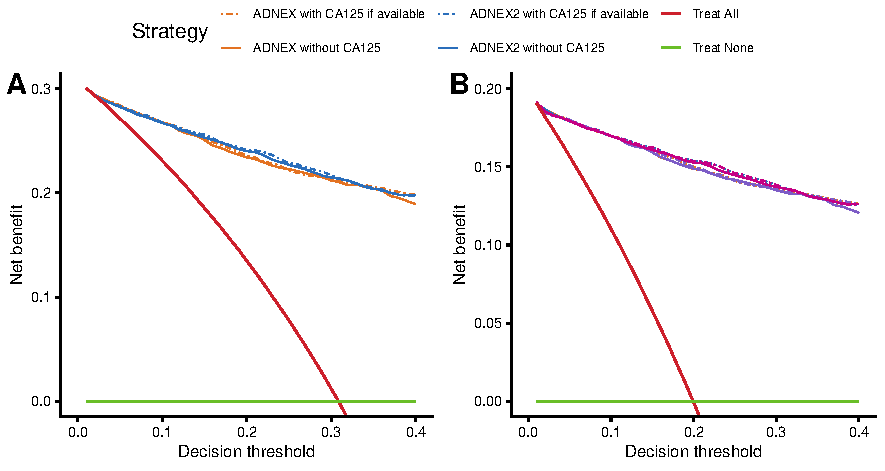
\includegraphics[width=0.8\textwidth]{figures/ADNEX2/DCA_combined_full.pdf}
\caption[Decision curves for ADNEX2 and ADNEX]{Decision curves for ADNEX2 and ADNEX in patients where BDs did not apply (n = 4657) (A) and in the two-step strategy with ADNEX2 or ADNEX (n = 6847) (B).}
\label{fig:ADNEX2:3}
\end{figure}

\subsection{Subgroup analysis}

Predefined subgroups were based on menopausal status (premenopausal vs postmenopausal), type of centre (oncology vs non-oncology) and a subgroup defined as patients that were operated within 120~days after inclusion scan. The \glsentryshort{AUC}s of the two step strategy with ADNEX2 or \gls{ADNEX} ranged from 0.91 to 0.95 (Figure S49). AUCs were higher in postmenopausal than in premenopausal patients and in oncology than in non-oncology centres. Pairwise AUCs in the subgroup of patients operated within 120 days showed similar performance to the performance in the whole population (Table S16). The discrimination of the two step strategy with ADNEX2 or ADNEX showed identical results. Forest plot for the two step strategy with ADNEX2 in all subgroups are included in Figures S50-S59. Predicted risks where underestimated across all subgroups, with slightly better calibration in non-oncology centres (Figures S60-S79). Calibration was more heterogeneous between centres among oncology centres than among non-oncology centres, as indicated by the wider prediction intervals (Figures S72-S79). Calibration was better but slightly more heterogeneous for ADNEX2 than for ADNEX across all subgroups. The number of cases in the subgroups was too low to perform multinomial calibration. 

For the 10\% threshold, sensitivity ranged between 0.85 and 0.96 and specificity between 0.72 and 0.89 (Table S17). For the 1\% threshold, the sensitivity ranged between 0.91 and 0.99 and specificity between 0.31 and 0.61 (Table S17). The two-step strategy with ADNEX2 showed clinical utility across the whole range of decision thresholds from >1\% to 40\%  in all subgroups, with comparable performance irrespective if CA125 was used or not (Table S18, Figure S80). However, at the 1\% decision threshold the utility was lower than the strategy of treating all patients. The proportion of centres in which the two-step strategy has clinical utility varied between 45\% and 84\% for the 1\% decision threshold and between 89\% and 97\% for the 10\% decision threshold. Clinical utility was higher in postmenopausal patients than premenopausal patients and in oncology centres rather than non-oncology centres. Clinical utility of the two-step strategy with ADNEX was similar to with ADNEX2 across all subgroups. 

\begin{table}
\centering
\tiny
\caption[Performance measures of ADNEX2 and ADNEX]{Summary of performance measures of ADNEX and ADNEX2 in the different populations and strategies. 10\% decision threshold was used for Sensitivity, Specificity, Net Benefit and p-useful.}
\label{tab:ADNEX2:2}
 \begin{tabularx}{\textwidth}{p{2cm}XXXXp{0.75cm}p{1.05cm}}
    \toprule
       \textbf{Model} & \textbf{AUC (CI)} &  \textbf{OE (CI)} & \textbf{Sensitivity (CI)} & \textbf{Specificity (CI)} & \textbf{Δ NB} & \textbf{P-useful} \\ 
        \midrule
        \multicolumn{7}{c}{Where benign descriptors do not apply (N = 4657)}  \\ 
        \midrule

        ADNEX2 without CA125 & 0.92 (0.90-0.93)  & 1.05 (0.96-1.14) & 0.95 (0.92-0.97) & 0.68 (0.63-0.73) & 0.0365 & 92\% \\ 
        ADNEX2 with CA125 if available & 0.93 (0.91-0.94)  & 1.04 (0.93-1.14) & 0.95 (0.92-0.97) & 0.69 (0.64-0.74) & 0.0364 & 91\% \\ 
        ADNEX without CA125 & 0.92 (0.90-0.93) & 1.16 (1.08-1.24) & 0.94 (0.90-0.96) & 0.70 (0.64-0.75) & 0.0368 & 89\% \\ 
        ADNEX with CA125 if available & 0.93 (0.91-0.94)  & 1.13 (1.05-1.22) & 0.94 (0.90-0.96) & 0.71 (0.65-0.76) & 0.0365 & 90\% \\ 
        \midrule
        \multicolumn{7}{c}{All patients (N=6847)} \\ 
        \midrule

        BD+ADNEX2 without CA125 & 0.94 (0.93-0.95) & 1.05 (0.95-1.14) & 0.93 (0.89-0.95) & 0.83 (0.78-0.87) & 0.0596 & 98\% \\ 
        BD+ADNEX2 with CA125 if available & 0.95 (0.93-0.96)  & 1.04 (0.94-1.14) & 0.93 (0.89-0.95) & 0.84 (0.79-0.87) & 0.0594 & 97\% \\ 
        BD+ADNEX without CA125 & 0.94 (0.93-0.95)  & 1.16 (1.08-1.24) & 0.92 (0.87-0.95) & 0.84 (0.79-0.88) & 0.0594 & 97\% \\ 
        BD+ADNEX with CA125 if available & 0.95 (0.93-0.96) & 1.13 (1.05-1.22) & 0.92 (0.87-0.95) & 0.85 (0.80-0.89) & 0.0592 & 98\% \\ 
        ADNEX2 without CA125 & 0.94 (0.93-0.95)  & 1.04 (0.94-1.12) & 0.93 (0.89-0.95) & 0.83 (0.78-0.87) & 0.0596 & 98\% \\ 
        ADNEX2 with CA125 if available & 0.95 (0.93-0.96)  & 1.03 (0.92-1.13) & 0.92 (0.89-0.95) & 0.84 (0.79-0.87) & 0.0593 & 97\% \\ 
        ADNEX without CA125 & 0.94 (0.93-0.95)  & 1.14 (1.05-1.22) & 0.92 (0.87-0.95) & 0.84 (0.79-0.88) & 0.0594 & 97\% \\ 
        ADNEX with CA125 if available & 0.95 (0.93-0.96) & 1.11 (1.03-1.20) & 0.92 (0.87-0.95) & 0.85 (0.80-0.89) & 0.0593 & 98\% \\ 
        \bottomrule
    \end{tabularx}
    \noindent\begin{minipage}{\textwidth}
\raggedright\footnotesize
\addlinespace[0.5em]

AUC: Area Under the receiver operating characteristic curve, ECI: Estimated calibration index, CI: Confidence interval, OE: Observed over expected ratio, Δ NB: Delta Net Benefit calculated at the 10\% decision threshold. This is the net benefit of using the model minus the maximum net benefit of treat all or treat none, P-useful: Probability of being useful in a hypothetical new centre at the 10\% decision threshold. BD: Benign descriptors. 
\end{minipage}
\end{table}

\begin{sidewaystable}
\centering
\scriptsize
\caption[Multiclass discrimination of ADNEX2 and ADNEX]{Polytomous discrimination index and pairwise AUC performance of ADNEX2 and ADNEX to distinguish between outcome categories. Results are shown with 95\% confidence intervals.}
\label{tab:ADNEX2:3}
    \begin{tabularx}{\textheight}{X|XXXX|XXXX}
    \toprule
        ~ & \multicolumn{4}{c}{\textbf{Patients where BDs do not apply (N = 4657)}}  & \multicolumn{4}{c}{\textbf{All patients (N = 6847)}} \\ 
        \midrule
        
        ~ & ADNEX2 without CA125 & ADNEX2 with CA125 if available & ADNEX without CA125 & ADNEX with CA125 if available & 2SS with ADNEX2 without CA125 & 2SS with ADNEX2 with CA125 if available  & 2SS with ADNEX without CA125 & 2SS with ADNEX with CA125 if available \\ 
        \midrule

        PDI (95\% CI) & 0.66 (0.64-0.68) & 0.67 (0.65-0.69) & 0.66 (0.64-0.68) & 0.69 (0.67-0.71) & 0.74 (0.72-0.76) & 0.76 (0.74-0.79) & 0.74 (0.72-0.76) & 0.76 (0.74-0.78) \\ 
        \midrule
        Benign vs Borderline & 0.88 (0.86-0.90) & 0.88 (0.86-0.90) & 0.88 (0.86-0.89) & 0.88 (0.86-0.90) & 0.92 (0.91-0.94) & 0.93 (0.91-0.94) & 0.92 (0.90-0.93) & 0.92 (0.91-0.94) \\ 
        Benign vs Stage I & 0.93 (0.91-0.94) & 0.93 (0.91-0.95) & 0.93 (0.91-0.95) & 0.93 (0.91-0.95) & 0.96 (0.94-0.97) & 0.96 (0.94-0.97) & 0.96 (0.94-0.97) & 0.96 (0.94-0.97) \\ 
        Benign vs Stage II-IV & 0.97 (0.96-0.97) & 0.98 (0.97-0.98) & 0.97 (0.96-0.97) & 0.98 (0.97-0.98) & 0.98 (0.97-0.98) & 0.98 (0.98-0.99) & 0.98 (0.97-0.98) & 0.98 (0.98-0.99) \\ 
        Benign vs Metastatic & 0.95 (0.93-0.96) & 0.95 (0.93-0.96) & 0.94 (0.93-0.96) & 0.95 (0.93-0.96) & 0.96 (0.94-0.97) & 0.96 (0.95-0.97) & 0.96 (0.94-0.97) & 0.96 (0.95-0.97) \\ 
        Borderline vs Stage I & 0.79 (0.75-0.82) & 0.79 (0.75-0.82) & 0.76 (0.73-0.80) & 0.76 (0.72-0.79) & 0.79 (0.75-0.82) & 0.78 (0.75-0.82) & 0.76 (0.73-0.80) & 0.76 (0.72-0.79) \\ 
        Borderline vs Stage II-IV & 0.91 (0.89-0.92) & 0.93 (0.91-0.94) & 0.90 (0.88-0.92) & 0.92 (0.90-0.94) & 0.91 (0.88-0.92) & 0.92 (0.91-0.94) & 0.90 (0.88-0.92) & 0.92 (0.90-0.93) \\ 
        Borderline vs Metastatic & 0.88 (0.85-0.91) & 0.88 (0.85-0.91) & 0.87 (0.84-0.90) & 0.87 (0.84-0.90) & 0.88 (0.85-0.90) & 0.88 (0.85-0.90) & 0.87 (0.84-0.90) & 0.87 (0.84-0.90) \\ 
        Stage I vs Stage II-IV & 0.73 (0.70-0.77) & 0.82 (0.79-0.84) & 0.74 (0.70-0.77) & 0.82 (0.79-0.85) & 0.73 (0.70-0.77) & 0.82 (0.79-0.84) & 0.74 (0.70-0.77) & 0.82 (0.79-0.85) \\ 
        Stage I vs Metastatic & 0.73 (0.69-0.77) & 0.73 (0.69-0.77) & 0.72 (0.67-0.76) & 0.71 (0.67-0.76) & 0.73 (0.69-0.77) & 0.73 (0.69-0.77) & 0.71 (0.67-0.76) & 0.71 (0.67-0.75) \\ 
        Stage II-IV vs Metastatic & 0.65 (0.61-0.69) & 0.80 (0.76-0.83) & 0.66 (0.62-0.70) & 0.80 (0.77-0.83) & 0.65 (0.61-0.69) & 0.80 (0.76-0.83) & 0.66 (0.62-0.70) & 0.80 (0.77-0.83) \\ 
        \bottomrule
        \addlinespace[0.5em]
    \end{tabularx}
\footnotesize \raggedright BD: Benign descriptors, PDI: Polytomous discrimination index
\end{sidewaystable}

\section{Discussion}

\subsection{Principal findings}

This study presents the development and validation of ADNEX2, an updated version of the \gls{ADNEX} model. ADNEX2 presents three main improvements over the original \gls{ADNEX}. First, it is developed using recent data, thereby addressing potential population drift \cite{vancalsterThereNoSuch2023}. Second, the cohort includes patients managed conservatively via ultrasound follow-up and excludes patients where the mass is clearly benign as indicated by the \glspl{BD}. The inclusion of conservatively management tumours is critical, as a key purpose of the model is to identify candidates for follow-up (risk $<$1\%). Conversely, the exclusion of clearly benign cases improves clinical relevance, as models are rarely required when the diagnosis is subjectively obvious where the \glspl{BD} can correctly classify almost all masses \cite{landolfoBenignDescriptorsADNEX2023}. Third, updating \gls{ADNEX} on a sample that included both operated and non-operated patients, such as in the \gls{IOTA}5 study, removes the selection bias of only including surgically managed patients and its potentially negative consequences \cite{timmermanIOTAPhase52025}.

The performance of the two-step strategy with ADNEX2 has shown excellent results. The model achieves \glsentryshort{AUC}s of 0.94--0.95 depending on if \gls{CA125} is used or not (Table~\ref{tab:ADNEX2:2}). \gls{CA125} mainly improved the ability of the model to differentiate between Stage I and Stage II--IV cancers and between Stage II--IV and second metastatic cancers (Table~\ref{tab:ADNEX2:3}). With respect to calibration, the model showed slight underestimation of risks (Figure~\ref{fig:ADNEX2:2}). However, centre specific performance was heterogeneous. This is a common issue in calibration \cite{vanAmsterdamCausalViewpoint2024, guptaDevelopmentValidationISARIC2021,steyerbergAssessmentHeterogeneityIndividual2019,vancalsterValidationModelsDiagnose2020} and may be caused for a wide range of reasons: different case-mix, different clinical guidelines etc.

\subsection{Strengths and limitations}

The main strength of this study is the alignment of an already successful prediction model with how it is used in clinical practice. ADNEX2 is the first model to assess ovarian masses preoperatively including patients that were managed with ultrasound follow-up. This approach reduced selection bias based on having histopathology. Other strengths are the large sample size and the multicenter nature of the study. We validated the model using IECV (also referred to as leave centre out cross-validation) and then retrained in the whole population. Therefore, we presented externally validated model performance while still using all available information for ADNEX2 development \cite{dehondPerspectivesValidationClinical2023}.

A limitation of including patients managed through ultrasound follow-up is that it induces differential verification bias because histopathology is not available for everyone. We determine the outcome of tumours without histopathology based on results of ultrasound follow-up and on multiple imputation \cite{vancalsterValidationModelsDiagnose2020}. We argue that differential verification bias is much less problematic than selection bias by excluding patients managed with ultrasound follow-up.

A second limitation is the presence of missing values for serum \gls{CA125}. Measuring \gls{CA125} was encouraged, but not mandatory and left to local judgement. When developing ADNEX2, we handled the missing values with multiple imputation to develop ADNEX2 both with and without \gls{CA125} as a predictor. However, as opposed to other external validations, we validated ADNEX2 with a `\gls{CA125} if available' strategy. This strategy better reflects model use in clinic, where \gls{CA125} is not available for all patients.

A third limitation is that the performance of \gls{ADNEX} is slightly more optimistic than the performance of ADNEX2. We compared the IECV results of ADNEX2 with \gls{ADNEX}, indicating that ADNEX2 has slightly better calibration. For ADNEX2, every centre-specific result is a geographically validated result, whereas 11/17~centres were part of the \gls{ADNEX} development such that for 11~centres the \gls{ADNEX} result is a temporally validated result.

A last limitation is that model fairness could only be evaluated in terms of menopausal status, because IOTA5 does not include information about ethnicity or socioeconomical status.

\subsection{Comparison with other studies}

The reported \gls{AUC} of two-step strategy with ADNEX2 of 0.95 compares favourably with recent studies. A recent systematic review with meta-analysis of \gls{ADNEX} external validation studies found that only two studies validated \gls{ADNEX} on cohorts of patients that were managed either with surgery or with ultrasound follow-up Barreñada et al. (2024) \cite{barrenadaADNEXRiskPrediction2024}. Both for \gls{ADNEX} with and without \gls{CA125}, a summary \gls{AUC} for benign versus malignant tumours of 0.94 was reported based on 4,509~tumours from 17~centres for \gls{ADNEX} without \gls{CA125} and on 5,132~tumours from 18~centres for \gls{ADNEX} with \gls{CA125} Barreñada et al. (2024) \cite{barrenadaADNEXRiskPrediction2024}. 95\% \gls{PI} was 0.82--0.98 for \gls{ADNEX} without \gls{CA125} and 0.88--0.99 for \gls{ADNEX} with \gls{CA125}. Later, the ROCkeTS study validated \gls{ADNEX} in a cohort of patients from primary or secondary care with non-specific systems and either elevated \gls{CA125} or abnormal ultrasound that were either managed surgically or by ultrasound follow-up. ROCkeTS reported an \gls{AUC} of 0.83 (95\% \gls{CI} 0.78--0.87) in premenopausal patients and of 0.89 (0.86--0.91) in postmenopausal patients \cite{sundarRiskpredictionModelsPostmenopausal2024,sundarDiagnosticTestsOvarian2026}. In recent head-to-head comparisons, \gls{ADNEX} outperformed Risk of Ovarian Malignancy Algorithm (\gls{ROMA}) and \gls{RMI} in premenopausal and postmenopausal patients (Barreñada, Ledger, et al., 2025; Sundar et al., 2024, 2026). The performance of the two-step strategy has been validated seven times \cite{barcroftEvaluatingUseTwostep2024,borgesProspectiveExternalValidation2024, devitisDiagnosticAlgorithmsAdnexal2025, einigExternalValidationIOTA2025, pascualValidationADNEXIOTA2024,perryCostConsequenceAnalysis2026, timmermanExternalValidationOvarianAdnexal2023}, with studies reporting \glsentryshort{AUC}s of 0.91--0.95, in line with our results.

Deep learning on ultrasound images has emerged in the last years. In a systematic review, forty studies developing image-based models to estimate the risk of malignancy of ovarian tumours where found Geysels et al. (2025) \cite{geyselsArtificialIntelligenceApplied2025}. \glsentryshort{AUC}s between 0.75 and 0.99 were reported at internal validation, however 95\% studies were at high risk of bias. Most of these models were built only on patients that underwent surgery. One of these models has been externally validated in a prospective multicenter cohort, showing promising results Christiansen et al. (2025) \cite{christiansenInternationalMulticenterValidation2025}. The study reported an \gls{AUC} of 0.93 with very good calibration, but no measures of clinical utility were presented Van Calster et al. (2025) \cite{vancalsterPerformanceEvaluationPredictive2024}.

\subsection{Clinical implications and future research}

ADNEX2 is intended to be used as part of a two-step strategy (Figure~\ref{fig:ADNEX2:4}). When a patient presents with a newly detected mass, the \gls{BD} are first checked. If a descriptor applies, the estimated risk of malignancy is $<$1\% and ADNEX2 is not needed. The patient can be considered for conservative management. If the \gls{BD} do not apply, ADNEX2 is applied. At this point, we argue that \gls{CA125} measurement is not mandatory and the ADNEX2 version without \gls{CA125} can be used. If \gls{CA125} is available, however, we do recommend using the version with \gls{CA125}. If the model's overall estimated risk of malignancy is $<$1\%, the patient can be considered for conservative management. If the estimated risk is at least 1\% but less than 10\%, management using standard surgical techniques can be considered locally. If the estimated risk is at least 10\%, we recommend that the patient is referred to an oncology centre for advanced gynaecological care. There, the estimated risks of the four subtypes of malignancy should be considered to guide specific management. In this case, we recommend measuring \gls{CA125} if it was not yet available, and to obtain updated risks from the ADNEX2 version with \gls{CA125} as a predictor. Depending on the local context or preferences, the threshold of 10\% can be changed. If a patient is first seen in a non-oncology centre and then referred to an oncology centre, the type of centre predictor should change accordingly.

The two-step strategy involving \gls{BD} and ADNEX2 supports two decisions: the decision whether or not the patient should be managed conservatively and the decision whether or not the patient should be referred to a specialised centre for management by a gynaecological oncologist (Figure~\ref{fig:ADNEX2:4}).

The model can be externally validated freely using the evaluatr, which is a platform developed to ensure statistical disclosure control and provide aggregate performance without compromising the model coefficients or the patient's characteristics. However, to be safely used in a decision support tool in clinic, the model needs to be used through the application developed by Gynaia Inc, complying with local regulations.

More prospectively collected multicentre studies are needed to validate the performance of ADNEX2 in patients that are surgically managed or managed with ultrasound follow up. Validating ADNEX2 in cohorts where patients are surgically managed could also be useful, but we anticipate the model to underestimate risks in that subpopulation and the performance not reflecting the performance as used in clinic.

\section{Conclusion}

ADNEX2 is an important improvement over \gls{ADNEX} in the model-aided management of adnexal masses. The newly presented model is developed to work within the two-step strategy and including patients that are conservatively managed, improving calibration and reducing selection bias.

\begin{figure}
\centering
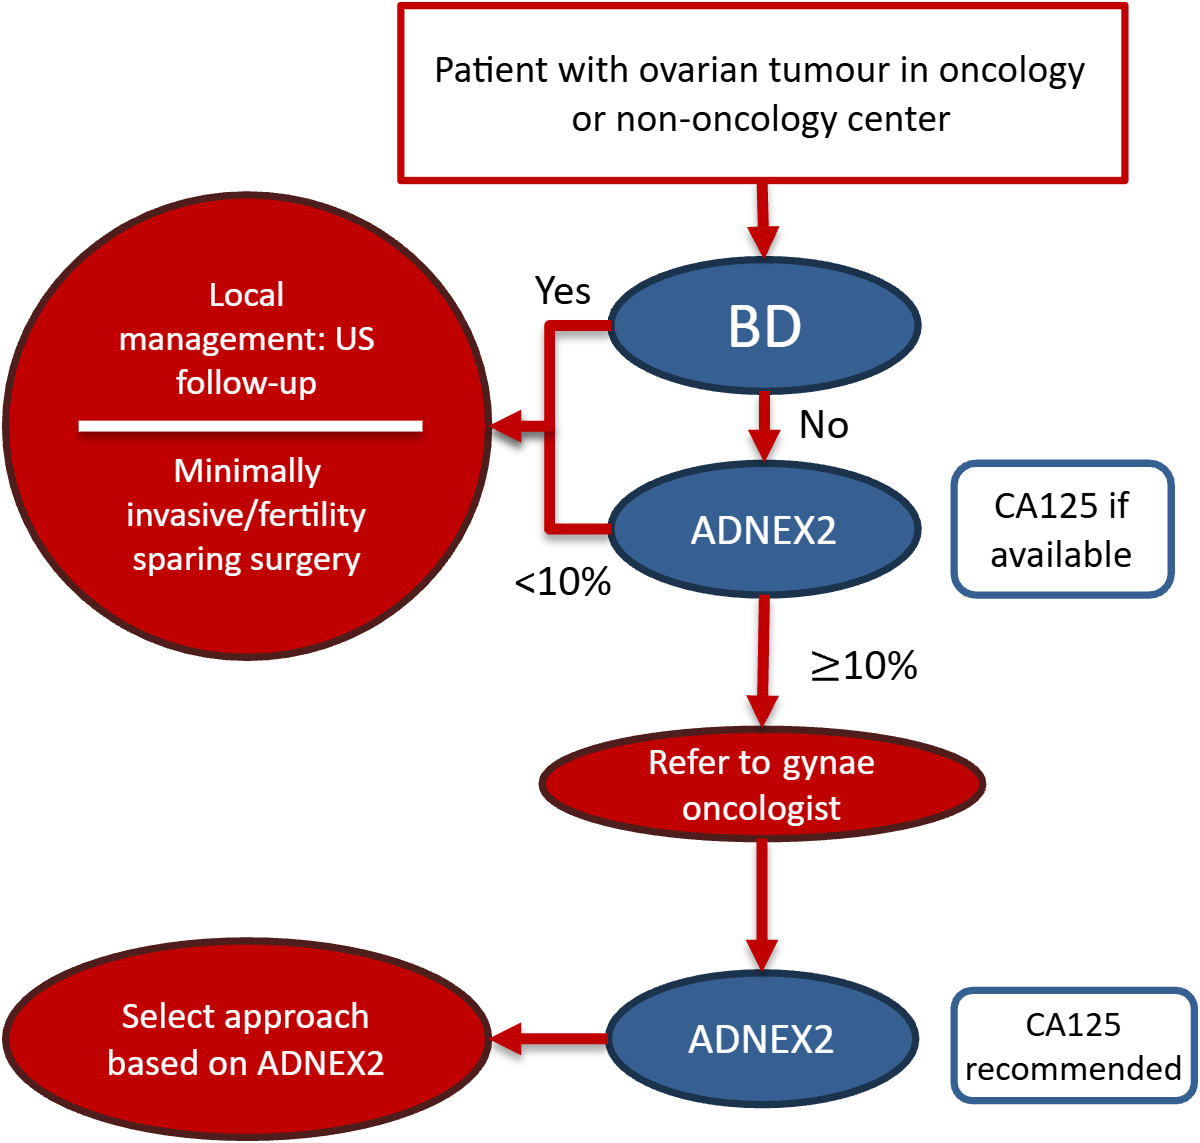
\includegraphics[width=0.8\textwidth]{figures/ADNEX2/Fig4.png}
\caption{Patient management diagram in two-step strategy with ADNEX2}
\label{fig:ADNEX2:4}
\end{figure}


\subsection*{Conflicts of interest}

DT and TB are co-founders of and have stock options in Gynaia Inc., a company providing teaching, training, data collection, and decision support tools (such as the ADNEX2 model) for clinicians and researchers in the field of gynecology. BVC and WF have stock options in Gynaia Inc. BVC and DT report consultancy work done by KU Leuven to help implement and test the original ADNEX model in ultrasound machines by Samsung Medison, Mindray, ESAOTE, and GE Healthcare, outside the submitted work. TB reports grants, personal fees, and travel support from Samsung Medison; travel support from Roche Diagnostics; and personal fees from GE Healthcare, all outside the submitted work. BVC, DT, WF, LW, LB and JC are co-inventors of ADNEX2  licensed to Gynaia Inc. and are entitled to inventorship rights. The other authors declare no conflict of interest.

\subsection*{Protocol}

The \gls{IOTA}5 protocol was registered in clinicaltrials.gov (\url{https://clinicaltrials.gov/study/NCT01698632}) and the statistical analysis plan was preregistered in an Open Science Foundation (\gls{OSF}) preregistration.

\subsection*{Data Sharing}

Follow-up data collection for the IOTA5 study is ongoing. When the study has closed and results have been published, the study responsible may share data upon reasonable request to dirk.timmerman@uzleuven.be. The R code and a dataset that includes centre code, outcome and patient risk of malignancy for each of the different models and strategies will be shared to allow readers to reproduce the results and figures.

\subsection*{Code sharing}
    
All code to produce the results and visualisations in the document will be shared in an \gls{OSF} repository.

\subsection*{Patient and public involvement}

The \gls{IOTA} group has a patient representative from Esperanza support group (\url{https://esperanza-lotgenotengroep.be/}), who is involved in the design and conduct of the studies. The patient representative is involved in the interpretation of the results and in the writing of the manuscript. The patient representative is also involved in the dissemination of the results to patients and the public.